\documentclass{report}
\usepackage{graphicx}
\usepackage{hyperref}
\usepackage{url}
\usepackage[left=25mm,right=25mm,top=25mm]{geometry}


\begin{document}

\title{Storyflow - Tracking the Evolution of Stories}
\author{Andreea Muscalagiu 1456893\\
Sorin Adrian Robert Davidoi		1456867}
\maketitle
\chapter{Problem definition}
\par
A narrative or story is any report of connected events, actual or imaginary, presented in a sequence of written or spoken words, or still or moving images \cite{Narrative}. Every story has characters who interact with each other and locations where events take place. The interaction of multiple characters between two adjacent time frames is a session. In a storyline visualization, these characters are represented as lines and relationships between them are proportional to the distance between their corresponding lines. Understanding how relationships between characters evolve over the course of the story is an interesting subject for various applications. Such applications could be analyzing tweets related to a particular story or the plot of a movie.

\par The paper Storyflow - Tracking the Evolution of Stories by Liu et al. deals with creating visualizations that help users better analyze a story, particularly the connections between characters and locations. By considering algorithms and techniques included in the paper, our task was to provide a visualization that facilitates this analysis. The result should be aesthetically pleasing, easy to follow, interactive and it should support hierarchical locations and the rendering of a large number of characters. This can be achieved by minimizing 4 metrics: line crossings, line wiggles, wiggle distance and white space. Line crossings create visual clutter and may lead to occlusion. Line wiggles represent how straight the lines are. The reason to minimize them is that wiggled lines are harder to follow and increase the visual clutter. Wiggle distance is related to line wiggles. Minimizing it leads to a more compact layout. The last metric, white space, is minimized in order not to waste screen space or have an unbalanced layout.

\par
The optimization problem is split into two parts: discrete optimization to minimize the first 2 metrics and continuous optimization to minimize the last 2 metrics. Minimizing the number of line crossings affects the visualization mostly, so it is the first step in the algorithm and it consists of ordering lines, sessions and locations such that there is minimum occlusion. The second step deals with aligning as many sessions and lines as possible between adjacent time frames. Finally, to generate a compact and pleasing storyline visualization, the wiggle distance and white space must be optimized. A set of interactions are also provided, according to the paper, such as adding, deleting, repositioning and straightening of lines, as well as bundling of sessions. To sum up, the user's tasks were the following:
\begin{itemize}
\item choose a data set to visualize
\item minimize line crossings
\item minimize line wiggles
\item minimize white space and wiggle distance
\item add real-time interaction
\end{itemize}

\chapter{Our Approach}
\par
We have decided to implement at least a part of the algorithms for optimizing the storyline visualization and also add some user interaction, such as highlighting one or more characters, choosing which characters to visualize, choosing a data set. The algorithm we have chosen to implement is the ordering algorithm, which involves minimizing line crossings in 2 steps: sorting locations and ordering sessions and lines. We would like to obtain a good initial layout. We did this by reading a reference paper \cite{4308636} where a graph sweeping algorithm is described and by extending this technique. It involves computing the ordering of every next time frame according to the previous time frame. After that, the time frames are traversed from the end to the beginning. This sweeping is done for a maximum number of iterations which we have chosen. At every step, the barycenter method presented in the paper is used for sorting the characters and the sessions.
\par
We follow the rules regarding how to represent characters and their relationships. Additionally, we have added a representation for locations as colored closed contours around the characters in that location. We have used the data sets provided on Tanahashi's website \cite{website:tanahashi} and transformed them into the JSON format.

\chapter{Related Work}
\centerline{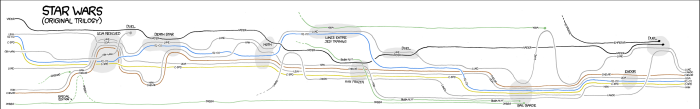
\includegraphics{movie_narrative_chart_star_wars_resized}}
\par
Such a storyline visualization was first introduced by R. Munroe through his movie narrative chart \cite{xkcd}. The lines of the characters run from left to right and their relationships are mapped to the distance between their lines at every time frame. Lines are adjacent when characters are in the same location. This visualization was drawn by hand and has lead to research on automatically generating a storyline layout.
\par
An existing visualization technique, designed by Tanahashi and Ma \cite{tanahashi} produces a pleasant-looking storyline visualization. Unfortunately, it takes too much time, when having a large number of characters, because it is based on a genetic algorithm. Therefore, no user interaction is provided. The implementation in Python and the data sets are available on Tanahashi's website \cite{website:tanahashi}.

\chapter{Implementation}
\par
In our implementation we have decided to use Javascript and create the visualizations using D3. The two important parts of our program are the algorithm that orders the locations, sessions and characters and the actual visualization. In the function buildDrawStoryFlow, the two important functions are called, which are annotateDataset and drawStoryFlow, the first one being responsible with the algorithm, and the second with the drawing of the storyline.

\section{Visualization}
\par
For our visualization, we have a few options that we can change, such as the interpolation function for drawing the lines, how thick the lines should be, how thick they should be when highlighted, the duration of transition from viewing all the lines to highlighting one or more particular lines, opacity of non-highlighted lines and maximum number of iterations, which is strictly concerned with the algorithm.
\par
In the function drawStoryFlow we set attributes necessary for visualizing the character lines, such as color and coordinates. We need to scale our time frame to the screen and compute the path of each character.
Because one might want to follow the journey of one or more particular characters in order to analyze their relationship, we have implemented character highlighting. When you click on one or more characters, the others fade away and the lines of the selected ones are thickened. They can be deselected by clicking on the background area. This is done using transitions, which switch from one stroke width to another, respectively from one opacity to a different one.

\section{Ordering algorithm}
\par
Because we found the algorithms presented in the paper quite complex, we have focused only on minimizing the most important metric, which is represented by the line crossings. This is done in the function annotateDataset using an ordering algorithm in 2 steps: ordering the locations and ordering the sessions and characters.
\par
In the function enforceHierarchy, first we compute the story time frame and then we sort the locations by the number of characters that are in the location during the movie, the first ones being the locations with the most characters. Normally, we would have to only place the first location with the most characters and place the rest according to the number of crossings, but we have chosen an easier approach. At some point, for every location we need to sort the sessions by their weights, which are considered to be their order in the list of sessions in that location.
\par
We need one relationship tree for every time frame, so we build it. We add every location and each location contains the sessions that take place in that location. We call the function enforceHierarchy for every time frame.
\par


\chapter{Conclusion}
\par
In conclusion, we consider that creating visualizations using D3 is a satisfying activity, given that it takes little effort to obtain considerable results, while the algorithmic part is rather frustrating because of the difficulty with manipulating matrices in JavaScript. Still, we would like to try to implement the rest of the optimization techniques in order to see how they improve the layout of our visualization. We would like to add that we found it difficult to understand a scientific paper, and especially reproduce the steps described in it, as the authors are not always specific in their explanations. It would've been very useful to have an open source version of the algorithm in some programming language in order to compare the solutions and make sure that we understood the steps to be followed.

\bibliographystyle{plain}  
\bibliography{bibliography}

\end{document}